% !TEX root = ./Vorlesungsmitschrift DIFF 2.tex  
\lecture{Mo 15.06. 10:15}{}
Letztes Mal: Existenz- und Eindeutigkeitssatz.

Die Forderung an \( F \), lokal einer Lipschitz-Bedingung zu genügen, ist wichtig, wie folgendes Beispiel zeigt:
\begin{beispiel*}
  \( x'=x^{\frac{2}{3}} \), \( x(t_0)=0 \). Dieses AWP hat Lösungen
  \begin{align*}
    u(t)&=0\quad \forall t\\
    u(t)&=\frac{1}{27}(t-t_0)^3\quad \forall t\\
    u(t)&=\begin{cases}
      \frac{1}{27}(t-a)^3\quad t\leq a\\
      0&a\leq t\leq b\\
      \frac{1}{27}(t-b)^3 t\geq b
    \end{cases}
  \end{align*}
  für beliebige \( a<t_0<b \).

  \( F(t,x)=x^{2/3} \) erfüllt zwar lokal bei \( (t_0,x_0) \), \( x_0\neq 0 \), eine Lipschitzbedingung (\( \partial_2 f(t,x)=\frac{2}{3}x^{-\frac{1}{3}} \) ist für \( x\neq 0 \) stetig) aber nicht bei \( (t_0,0) \) (für kein \( t_0 \)).

  Der Beweis des Satzes von Picard + Lindelof war konstruktiv, \dh man kann ihn (wenn lokal eine Lipschitz-Bedingung erfüllt ist) verwenden, um Lösungen zu finden (siehe letzte Mal).

  In diese Vorlesung lernen wir Verfahren kennen, die auch in anderen Fällen Lösungen liefern.
\end{beispiel*}
\begin{lemma}\label{dgl_mit_getrennten_variablen}
  Seien \( G\maps \tilde{J}\to \reals \), \( H\maps J\to \reals \), stetig, \( J,\tilde{J} \) Intervalle. Sei \( G(x)\neq 0\quad \forall x\in \tilde{J} \). 
  Betrachte 
  \begin{align*}
    \tilde{H}(t)&=\Integrate{H(s)}{s,t_0,t}\\
    \tilde{G}(x)&=\Integrate{\frac{1}{G(y)}}{y,u_0,x}.
  \end{align*}
  Ist \( t_0\in I \) mit \( I\subset J \) und \( \boxed{\tilde{H}(I)\subset\tilde{G}(\tilde{J})} \). Dann hat die Differentialgleichung
  \begin{equation*}
    x'=F(t,x),\quad F\maps J\times \tilde{J}\to \reals,\logicspace F(t,x)=H(t)\cdot G(x)
  \end{equation*}
  (\enquote{Differentialgleichung mit \emph{getrennten Variablen}}) mit der Anfangsbedingung
  \begin{equation*}
    x(t_0)=u_0, \quad (t_0,u_0)\in I\times \tilde{J}
  \end{equation*}
  eine eindeutige Lösung \( u\maps I\to \reals \), \( I\subset J \).
\end{lemma}
\begin{proof}
  \begin{itemize}
    \item Ist \( u\maps I\to \reals \) Lösung des AWP, so gilt 
    \begin{equation*}
      \tilde{G}(u(t))=\tilde{H}(t) \quad \forall t\in I.
    \end{equation*}
    Denn: Aus \( u'(s)=H(s) G(u(s)) \) folgt
    \begin{equation*}
      \equalto{(\text{Substitutionsregel})\ \Integrate{\frac{1}{G(u)}}{u,u_0,u(t)}}{\Integrate{\frac{u'(s)}{G(u(s))}}{s,t_0,t}}=\Integrate{H(s)}{s,t_0,t}.
    \end{equation*}
    Insbesondere ist also \( I \) derart, dass \( \tilde{H}(I)\subset \tilde{G}(\tilde{J}) \).
    \item \( \tilde{G}'(x)=\frac{1}{G(x)}\neq 0 \) \timplies \( \tilde{G}  \) ist streng monoton \timplies \( \tilde{G} \) besitzt \( \stetigefunktionen[1] \) Umkehrfunktion \( \inverse{\tilde{G}}\maps \tilde{G}(I)\to \reals \) \timplies mit dem eben bewiesenen
    \begin{equation*}
      u(t)=\inverse{\tilde{G}}(\tilde{H}(t))\tag{\( * \)}\label{eq:dgl_mit_getrennten_variablen:berechnung_loesung}
    \end{equation*}
    \timplies Wenn sie existiert, ist die Lösung eindeutig.
    \item Existenz: Wir nehmen \eqref{eq:dgl_mit_getrennten_variablen:berechnung_loesung} als Definition und zeigen, dass \( u \) dann das AWP löst.\( u \) ist \( \stetigefunktionen[1]\) \checkmark, und wegen \eqref{eq:dgl_mit_getrennten_variablen:berechnung_loesung} gilt
    \begin{equation*}
      u(t_0)=\inverse{\tilde{G}}(\tilde{H}(t_0))=\inverse{\tilde{G}}(0)=u_0,
    \end{equation*}
    sowie (\( \tilde{G}(u(t))=\tilde{H}(t) \))
    \begin{equation*}
      \tilde{G}(u(t))\cdot u'(t)=\frac{1}{G(u(t))}\cdot u'(t)=\tilde{H'}(t)=H(t)
    \end{equation*}
    \timplies \Beh.
  \end{itemize}
\end{proof}
\begin{merkregel}
  \begin{align*}
    \frac{\differential x}{\differential t}&=H(t) G(x)\\
    \frac{\differential x}{G(x)}&=H(t)\differential t.\\
    \Integrate{\frac{1}{G(x)}}{x}=\Integrate{H(t)}{t}.
  \end{align*}
  Dem kann man tatsächlich einen Sinn geben --- Stichword Differenzialformen.
\end{merkregel}
\begin{bemerkung*}
  Wir haben im Beweis gesehen: Jede Lösung einer DGL mit getrennten Variablen erfüllt
  \begin{equation*}
    \tilde{G}(u(t))=\tilde{H}(t)\quad \forall t\in I.
  \end{equation*}
  Das kann man nutzen, um die Lösung zu bestimmen.
\end{bemerkung*}
\begin{beispiel*}
  \( x'=x^2 \), \( x(0)=c \), \( c\in\reals \). Eindeutige Lösung nach \thref{dgl_mit_getrennten_variablen} mit \( I \) wie dort oder wegen der lokal erfüllten Lipschitz-Bedingung.
  \begin{description}
    \item[\( c=0 \)] \( u(t)=0\quad \forall t\in \reals \).
    \item[\( c>0 \)] Sei \( u\maps I\to \reals \) eine Lösung mit \( u(0)=c>0 \). Dann ist \( u(t)>0 \quad \forall t\in I\) (denn gäbe es \( t_{*} \) \sd \( u(t_{*})=0 \), wäre wegen der Eindeutigkeit \( u(t)=0\quad \forall t \) (auch für \( t=t_0 \))). Betrachte also \( F\maps \reals\times\reals_{>0}\to \reals \), \( F(t,x)=x^2 \). Berechne 
    \begin{align*}
      \tilde{H}(t)=\Integrate{}{s,0,t}=t\\
      \tilde{G}(x)=\Integrate{\frac{1}{y^2}}{y,c,x}=\frac{1}{c}-\frac{1}{x}.
    \end{align*}
    \( \tilde{G}(\reals_{>0})=\ointerval{-\infty}{\frac{1}{c}} \). Setze also \( I=\ointerval{-\infty}{\frac{1}{c}} \) (\sd \( \tilde{H}(I)=I\subset \tilde{G}(\reals_{>0}) \)). Für eine Lösung der AWP gilt nach \thref{dgl_mit_getrennten_variablen}
    \begin{equation*}
      \frac{1}{c}-\frac{1}{u(t)}=t\quad \forall t\in I.
    \end{equation*}
    \timplies \( u(t)=\frac{c}{1-ct} \) und \( t<\frac{1}{c} \).
    \item[\( c<0 \)] Genauso:
    \begin{equation*}
      u(t)=\frac{c}{1-ct}
    \end{equation*}
    und \( t>\frac{1}{c} \).
  \end{description}
\end{beispiel*}
\begin{beispiel*}
  Logistisches Wachstum \( x'=\alpha x(1-x) \), \( \alpha>0 \) auf \( \reals\times \ointerval{0}{1} \) (\( G(x)=x(1-x)\neq 0 \quad \forall x\in \ointerval{0}{1}\)). Seperation der Variablen:
  \begin{equation*}
    \equalto{\evaluatebetween{\Ln{\abs*{\frac{y}{y-1}}}}{x_0}{u(t)}\ \parens*{\text{Partialbruchzerlegung: } \frac{1}{y(1-y)}=\frac{1}{y}-\frac{1}{y-1}}}{\Integrate{\frac{1}{y(1-y)}}{y,x_0,u(t)}}\needed{=}\Integrate{\alpha}{s,t_0,t}=\alpha(t-t_0).
  \end{equation*}
  Also \( \frac{u(t)}{u(t)- 1}=\pm e^{\alpha t+C}  \), \( C \) Konstante.
  \begin{equation*}
    \implies u(t)=\frac{e^{\alpha t}}{\tilde{C}+ e^{\alpha t}}\quad (\tilde{C}=\mp e^C).
  \end{equation*}
  Anfangsbedingung \( u(0)=x_0 \), \( x_0\in \ointerval{0}{1} \). \( x_0\frac{1}{\tilde{C}+1} \), also \( \tilde{C}=\frac{1-x_0}{x_0}>0 \). Also ist \( u \) auf ganz \( \reals \) definiert.
\end{beispiel*}
\begin{lemma}\label{homogene_DGL}
  Sei \( f\maps I\to \reals \), (\( I\subset \reals \) Intervall) und sei
  \begin{equation}
    V=\set{(t,x)\in \explain{\reals\setminus \zeroset}{\fieldwithoutzero{\reals}}\times \reals|\frac{x}{t}\in J}.
  \end{equation}
  Betrachte das DGL
  \begin{equation*}
    \label{eq:homogene_DGL} x'=f\p*{ \frac{x}{t} }\tag{\( * \)}
  \end{equation*}
  auf \( V \). Dann gilt \( u\maps I\to \reals \), \( I\subset \fieldwithoutzero{\reals} \) Intervall, ist genau dann Lösung von \eqref{eq:homogene_DGL} zur Anfangsbedingung \( x(t_0)=x_0 \), \( t_0\in I \), \( (t_0,x_0)\in V \), wenn \( v(t)\definedas \frac{u(t)}{t} \) Lösung des AWP
  \begin{align*}
    y'&=\frac{1}{t}(f(y)-y)\\
    y(t_0)&=\frac{x_0}{t_0}
  \end{align*}
  ist.  
\end{lemma}
\begin{bemerkung*}
  Man sagt, die zweite DGL gehe durch Substitution aus der ersten hervor. Merkregel:
  \begin{equation*}
    y=\frac{x}{t},\quad y'=\frac{x'}{t}-\frac{1}{t^2}x=\frac{1}{t}\parens*{f\parens*{\frac{x}{t}}-\frac{x}{t}}.
  \end{equation*}
  Die \ordinalnum{2} DGL ist lösbar wie in \thref{dgl_mit_getrennten_variablen}.
\end{bemerkung*}
\begin{proof}[Beweis von \ref{homogene_DGL}]
  \begin{proofdescription}
    \item[\hin] Sei \( u \) Lösung der \ordinalnum{1} GLeichung und \( u(t_0)=x_0 \). Dann ist 
    \begin{align*}
      v'(t)&=\frac{u'(t)}{t}-\frac{u(t)}{t^2}\\
      &=\frac{1}{t}f\parens*{\frac{u(t)}{t}}-\frac{u(t)}{t^2}
    \end{align*}
    und \( v(t_0)=\frac{x_0}{t_0} \).
    \item[\rueck] Sei \( v \) Lösung der \ordinalnum{2} Gleichung und \( v(t_0)=\frac{x_0}{t_0} \). Dann ist
    \begin{align*}
      u'(t)&=(t v(t))'=v(t)+t v'(t)\\
      &=v(t)+(f(v(t))-v(t))\\
      &=f(u(t)/t)
    \end{align*}
    und \( u(t_0)=x_0 \).
  \end{proofdescription}
  
\end{proof}
\begin{beispiel*}
  \( x'=1+\frac{x}{t}+\parens*{\frac{x}{t}}^2 \) auf \( \reals_{>0}\times \reals \). Substitution
  \begin{equation*}
    \rightsquigarrow y'=\frac{1}{t}(1+y^2).
  \end{equation*}
  Trennung der Variablen:
  \begin{gather*}
    \Integrate{\frac{1}{1+z^2}}{z,y_0,v(t)}=\Integrate{\frac{1}{s}}{s,t_0,t}\\
    \implies\ArcTan{v(t)}-\ArcTan{y_0}=\Ln{\frac{t}{t_0}},
  \end{gather*}
  also \( u(t)=t\cdot \Tan+*{\Ln{\frac{t}{t_0}}+a} \) löst die ursprüngliche Gleichung und ist auf einem Intervall \( I \), das \( t_0 \) enthält, definiert.
\end{beispiel*}
\begin{bemerkung*}
  Typische DGL aus der klassischen Mechanik (Physik)
  \begin{equation*}
    x''=f(x)\tag{*}\label{kraft_dgl},
  \end{equation*}
  \( f\maps I\to  \reals \), \( I\subset \reals \) Intervall, stetig (\enquote{Kraft}). Definiere \( \underline{U}(x)=-\Integrate{f(s)}{s,a,x} \), \( \underline{U}\maps I\to \reals \) (\enquote{potentielle Energie}). Damit schreibt sich \( \eqref{kraft_dgl} \) wie folgt:
  \begin{equation*}
    x''=-\underline{U}'(x).
  \end{equation*}
  Ist \( w\maps J\to \reals \) Lösung, so gilt
  \begin{align*}
    \parens*{\frac{1}{2}w'(t)}^2&=w'(t)\cdot w''(t)\\
    &=w'(t)\cdot (-\underline{U}'(w(t)))\\
    &=-\frac{\differential}{\differential t}(\underline{U}\circ w)(t),
  \end{align*}
  also
  \begin{equation*}
    \frac{\differential}{\differential t}\parens[\big]{\frac{1}{2}w'(t)^2+\underline{U}(w(t))}=0
  \end{equation*}
  (Konstante der Bewegung). \timplies \texists Konstante \( E \) (\enquote{Gesamtenergie}) \sd
  \begin{equation}
    \frac{1}{2}v(t)^2+\underline{U}(w(t))=E\quad \forall t
  \end{equation}
  (\( v(t)=w'(t) \) \enquote{Geschwindigkeit})
  \timplies Lösungen müssen derart sein, dass \( \underline{U}(x(t))\leq E \) und es gilt dann
  \begin{equation*}
    w'(t)=\pm \sqrt{2(E-\underline{U}(w(t)))}
  \end{equation*}
  (je nachdem, ob \( w'\geq 0 \) oder \( \leq 0 \)).

  Wir betrachten also die DGL mit getrennten Variablen
  \begin{equation*}
    x'=\pm \sqrt{2(E-\underline{U}(x))}.
  \end{equation*}
\end{bemerkung*}
Oft sind DGL'n auch \emph{implizit} gegeben, also von der Form
\begin{equation*}
  f(t,x)+h(t,x)x'=0.
\end{equation*}
\begin{satz}[Exakte Differentialgleichungen]\label{exakte_dgl}\index{Exakte Differentialgleichungen}
  Sei \( f(t,x)+h(t,x)x'=0 \) gegeben, \( f \) und \( h\maps V\to \reals \) \( \stetigefunktionen[1] \), \( V=J_1\times J_2 \) mit \( J_1,J_2 \) Intervalle. Es gelte \( \partial_1 h=\partial_2 f \) auf \( V \). Dann gibt es eine zweimal stetig differenzierbare Funktion \( F\maps V\to \reals \) mit \( h=\partial_2 F \) und \( f=\partial_1 F \).

  Ist \( u\maps I\to \reals \) mit \( \Gamma_u\subset V \) eine Lösung der DGL, so gilt \( F(t,u(t)) =C\) (\( C \) durch Anfangsbedingung festgelegt). 

  Umgekehrt: Ist \( h(t_0,x_0)\neq 0 \), so ist \( F(t,x)=C \) lokal bei \( (t_0,x_0) \) auflösbar nach \( x \) und die Auflösungsfunktion \( u\maps I\to \reals \) löst die Differentialgleichung mit \( u(t_0)=x_0 \).
\end{satz}
\begin{proof}
  Dass \( \partial_1 h=\partial_2 f \) notwendig ist für die Existenz von \( F \) ist klar. Dass sie auch hinreichend ist, werden wir im letzten Teil der Vorlesung beweisen.

  Satz über implizite Funktionen: Betrachte \( F(t,x)-C=0 \). Ist \( \partial_2 F(t_0,x_0)\neq 0 \), so gibt es lokal bei \( (t_0,x_0) \) eine Auflösungsfunktion \( u\maps I\to \reals \), \( u(t_0)=x_0 \) mit
  \begin{equation*}
    u'(t)=-\inverse{\parens{\partial_2 F(t,u(t))}}\partial_1 F(t,u(t))\quad \forall t\in I,
  \end{equation*}
  also
  \begin{equation*}
    f(t,u(t))+h(t,u(t))\cdot u'(t)=0\quad \forall t\in I.
  \end{equation*}

  Ist umgekehrt \( u\maps I\to \reals \) Lösung der DGL, so gilt (mit \( \varphi(t)\definedas (t,u(t)) \))
  \begin{align*}
    (F\circ \varphi)'(t)&=\begin{pNiceMatrix} \partial_1 F(\varphi(t)) & \partial_2 F(\varphi(t)) \end{pNiceMatrix}\matrixmult \begin{pNiceMatrix} 1 \\ u'(t) \end{pNiceMatrix}\\
    &=f(t,u(t))+h(t,u(t))u'(t)=0.
  \end{align*}
\end{proof}
\begin{beispiel*}
  \begin{gather*}
    7t+7x+(6t-2x)x'=0\\
    \partial_t (6t-2x)=6=\partial_x (7t+6x)\\
    \partial_2 F=h\implies \Integrate{h(t,x)}{x}=F(t,x)+\tilde{C}(t)\\
    \implies F(t,x)=6tx-x^2+C(t)\\
    \partial_1 F=f\implies 7t+6x\needed{=}6x+C'(t)\\
    \implies C(t)=\frac{7}{2}t^2+C_0.
  \end{gather*}
  Allgemeine Lösung gegeben durch
  \begin{equation*}
    F(t,x)=\frac{7}{2}t^2+6tx-x^2=C,
  \end{equation*}
  also \( u(t)=3t\pm \sqrt{-C+25\frac{t^2}{2}} \), falls \( c>0 \), \( t>\frac{\sqrt{2c}}{5} \).

  Hyperbeln mit Hauptachsenrichtungen \( \begin{pNiceMatrix} 2 \\ 1 \end{pNiceMatrix} \) und \( \begin{pNiceMatrix} -1 \\ 2 \end{pNiceMatrix} \).
  \begin{figure}[H]
    \centering
    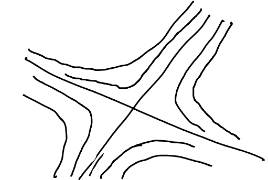
\includegraphics[width=0.5\linewidth]{exakte_dgl_hyperbeln}
    \label{fig:exakte_dgl_hyperbeln}
  \end{figure}
\end{beispiel*}
\begin{bemerkung*}
  Ist eine DGL der Form
  \begin{equation*}
    f(t,x)+h(t,x)x'=0
  \end{equation*}
  nicht exakt, kann man nach einer Funktion \( M \) suchen, \sd 
  \begin{equation*}
    M(t,x)f(t,x)+M(t,x)h(t,x)x'=0
  \end{equation*}
  exakt ist. Diese DGL hat dieselbe Lösungsmenge wie die ursprüngliche DGL\@. Eine solche Funktion \( M \) heißt \emph{Eulerscher Multiplikator}.

  Er muss erfüllen:
  \begin{equation*}
    \partial_2 M \cdot f+ M \partial_2 f=\partial_1 M\cdot h+M\partial_2 h,
  \end{equation*}
  also
  \begin{equation*}
    \partial_2 M\cdot f- \partial_1 M\cdot h+(\partial_2 f- \partial_1 h)M=0.
  \end{equation*}
\end{bemerkung*}
\begin{beispiele*}
  \begin{itemize}
    \item Wenn \( \frac{\partial_2 f --\partial_1 h}{h}=\rho(t) \) (unabhängig von \( x \)), kann man \( M(t)=Ce^{\Integrate{\rho(s)}{s,t_0,t}} \) wählen.
    \item Analog wenn \( \frac{\partial_1 h-\partial_2 f}{f}=\rho(x) \), kann man \( M(x)=Ce^{\Integrate{\rho(y)}{y,x_0,x}} \) wählen.
  \end{itemize}
\end{beispiele*}
\section{Lineare Differentialgleichungen}
\begin{definition}\label{homogenes_lineares_dgl_system}\index{Homogenes lineares DGL-System}
  Sei \( I\subset \reals \) ein Intervall und 
  \begin{equation*}
    A=\begin{pNiceMatrix} a_{11} & \Cdots & a_{1n} \\ \Vdots &  & \Vdots \\ a_{n1} & \Cdots & a_{nn} \end{pNiceMatrix}\maps I\to \sqmatrices{n}{\reals}
  \end{equation*}
  stetig (wir wir gesehen haben, ist dies gleichbedeutend mit der Stetigkeit aller \( a_{ij} \)). Dann heißt
  \begin{equation*}
    x'=A(t)x
  \end{equation*}
  \emph{homogenes (nicht im Sinne von \ref{homogene_DGL}) lineares Differentialgleichungssystem} (oder homogene lineare DGL) \emph{\ordinalnum{1} Ordnung}. Sei \( b=\begin{pNiceMatrix} b_1 \\ \Cdots \\ b_n \end{pNiceMatrix}\maps I\to \reals^n \) stetig (also alle \( b_i \) stetig). Dann heißt
  \begin{equation*}
    x'=A(t)x+b(t)
  \end{equation*}
  \emph{inhomogenes lineares Differentialgleichungssystem} (oder inhomogene lineare DGL) \emph{\ordinalnum{1} Ordnung}. Eine Lösung ist eine differenzierbare Funktion
  \begin{equation*}
    u\maps J\to \reals^n \logicspace \text{\sd}\logicspace u'(t)=A(t)\explain{\text{Matrix-Vektor-Multiplikation}}{\matrixmult} u(t)
  \end{equation*}
  \bzw \( u'(t)=A(t)\matrixmult u(t)+b(t) \).
\end{definition}
\begin{bemerkung*}
  Es gibt zum AWP
  \begin{equation*}
    x'=A(t)x+b(t),\quad x(t_0)=x_0
  \end{equation*}
  stets eine eindeutige Lösung
  \begin{equation*}
    u\maps J\to \reals^n, \quad u(t_0)=x_0.
  \end{equation*}
  Denn: Für \( F(t,x)=A(t)\matrixmult x+b(t) \) gilt
  \begin{equation*}
    \norm{F(t,x)-F(t,\tilde{x})}=\norm{A(t)\matrixmult(x-\tilde{x})}\leq C\explain{\sup_{v\neq 0}\frac{\norm{A(t)v}}{\norm{v}}}{\operatornorm{A(t)}}\cdot\norm{x-\tilde{x}}
  \end{equation*}
  und \( \sup_{t\in \interval{-\varepsilon+t_0}{t_0+\varepsilon}}<\infty \), da \( \interval{-\varepsilon+t_0}{t_0+\varepsilon} \) kompakt ist und \( t\mapsto \operatornorm{A(t)} \) stetig. 

  Wir werden sehen, dass eine lineare DGL immer eine Lösung besitzt mit \( J=I \).
\end{bemerkung*}
\begin{bemerkung*}
  Es ist zweckmäßig, auch komplexe lineare DGL'n zuzulassen, also \( A\maps I\to \sqmatrices{n}{\complexs} \), \( b\maps I\to \complexs^n \). Um Stetigkeit von \( A \) un \( b \) in diesem Fall zu definieren, identifiziert man \( \complexs=\reals^2 \), betrachtet also \( A \) als ABbildung mit Werten in \( \reals^{(2n)^2} \), \( b \) als Abbildung mit Werten in \( \reals^{2n} \). Dito für die Differenzierbarkeit von \( u \).
\end{bemerkung*}
Bevor wir den allgemeinen Fall studieren, betrachten wir \( n=1 \).
\begin{beispiel}
  \( a\maps I\to \reals \) stetig, \( x'=a(t)x \), \( x(t_0)=u_0 \). Das AWP hat die (eindeutige) Lösung
  \begin{equation*}
    u\maps I\to \reals,\quad u(t)=u_0\exp\parens*{\Integrate{a(s)}{s,t_0,t}}.
  \end{equation*}
  \( u(t) \) löst die Gleichung
  \begin{equation*}
    u'(t)=u_0\cdot a(t)\cdot \exp\parens*{\Integrate{a(s)}{s,t_0,t}}\quad \checkmark.
  \end{equation*}
\end{beispiel}
\begin{lemma}[\enquote{Variation der Konstanten}]\label{variation_der_konstanten}
  Betrachte \( x'=a(t)x+b(t) \), \( a,b\maps I\to \reals \) stetig, \( x(t_0)=x_0 \). Sei \( v\maps I\to \reals \) Lösung der zugehörigen homogenen GLeichung \( x'=a(t)x \). Sei \( v(t_0)\neq 0 \). Dann ist \( v(t)\neq 0\quad \forall t \) und wir erhalten die eindeutige Lösung \( u \) in der inhomogenen Gleichung vermöge
  \begin{equation*}
    u(t)\definedas v(t)\cdot w(t)
  \end{equation*}
  mit
  \begin{equation*}
    w(t)=\Integrate{\inverse{v(s)}b(s)}{s,t_0,t}+C,
  \end{equation*}
  wobei \( C \) so angepasst wird, dass \( u(t_0)=x_0 \) gilt.
\end{lemma}
\begin{proof}
  Wir machen den Ansatz \( u=v\cdot w \) und bestimmen \( w \). Es ist 
  \begin{align*}
    u'(t)&=v'(t)w(t)+v(t)w'(t)\\
    &=a(t)v(t)w(t)+v(t)w'(t)\\
    &=a(t)v(t)w(t)+b(t)\\
    \implies a(t)w'(t)&\needed{=}b(t)\implies \text{\Beh.}
  \end{align*}
  Denn \( v(t)\neq 0\quad \forall t \) wegen \( v(t_0)\neq 0 \) (denn wäre \( v(t_0)\neq 0 \) für ein \( t_{*} \) so wäre \( r(t)=0\quad \forall t \)).  
\end{proof}